\documentclass[xcolor=table,fontsize=10pt]{beamer}
% \usepackage[utf8]{inputenc}
% \usepackage[T1]{fontenc}
\usepackage{fontenc}

\usepackage{import}
\subimport{settings/}{general.tex}
\subimport{settings/}{colors.tex}
\subimport{settings/}{figures.tex}
\subimport{settings/}{math.tex}
% \subimport{settings/}{code.tex}
\subimport{settings/}{fonts.tex}
\subimport{settings/}{commands.tex}
\setbeamertemplate{navigation symbols}{
    \insertsectionnavigationsymbol\
    \insertsubsectionnavigationsymbol\
}

\newcommand{\blankitem}{\item[$\square$]}
\newcommand{\checkeditem}{\item[$\textcolor{green}{\checkmark}$]}
\newcommand{\plusitem}{\item[\faIcon{plus}]}
\newcommand{\shielditem}{\item[\faIcon{shield-alt}]}
\newcommand{\negitem}{\item[\red{\faIcon{minus}}]}

% Emoji support for LaTeX
\usepackage{emoji}
\setemojifont{Noto Color Emoji}
\usepackage{fontawesome5}
\usepackage{settings/mintcode}

% Importing images from another path
\graphicspath{{./images/}}

% Theme ------------------------------------------------------------------------
\usetheme{Antibes}
\usecolortheme{dolphin}
\setbeamercolor{structure}{fg=blue}
% \setbeamercolor{item}{fg=black}

% Title ------------------------------------------------------------------------
\title{\bft{Cloud Based Storage System}}
\subtitle{\small{\bft{CLOUD COMPUTING EXAM}}}
\author{Marco Tallone}
\date{September, 2024}

% \titlegraphic{
% 	
\includegraphics[width=0.2\textwidth]{sdic-logo.jpg}
% }
\titlegraphic{
    \begin{minipage}{0.45\textwidth}
        \centering
				
\includegraphics[width=0.5\textwidth]{sdic-logo.jpg}\\
				\small{\bft{SDIC} Master Degree}
    \end{minipage}
    \hfill
    \begin{minipage}{0.45\textwidth}
        \centering
				
\includegraphics[width=0.5\textwidth]{units.png}\\
				\small{\bft{U}ni\bft{TS}}
    \end{minipage}
}


% Document ---------------------------------------------------------------------
\begin{document}
\frame{\titlepage} % This creates a title slide

% SLides -----------------------------------------------------------------------

%-------------------------------------------------------------------------------
\section{Introduction}

\begin{frame}
	\frametitle{Introduction: Exam Exercises}

	% \only<1->{
		% \begin{block}{Exercise 1 \hfill \tiny{\bft{CLOUD BASIC}}}
		\begin{block}{Exercise 1 \hfill \raisebox{0.4ex}{\tiny{\bft{CLOUD BASIC}}}}
			Cloud Based Storage System with Docker Compose \hfill \faIcon{docker}
		\end{block}
	% }

	% \only<2->{
		\begin{block}{Exercise 2 \hfill \raisebox{0.4ex}{\tiny{\bft{CLOUD
			ADVANCED}}}}
			Cloud Based Storage System with Kubernetes \hfill \faIcon{dharmachakra}
		\end{block}
	% }

	% \only<3->{
		\begin{block}{Exercise 3 \hfill \raisebox{0.4ex}{\tiny{\bft{CLOUD
			ADVANCED}}}}
			OSU Latency Test on Kubernetes Cluster \hfill \faIcon{chart-line}
		\end{block}
	% }
\end{frame}
%-------------------------------------------------------------------------------
\section{Exercise 1}
%-------------------------------------------------------------------------------
\subsection{Assignment}

\begin{frame}[t]
	\frametitle{Exercise 1 Assignment}

		\begin{itemize}

			\only<1->{
				\item \bft{User authentication \emoji{key} and file management
					\emoji{file-folder}}
					\begin{itemize}
						\blankitem\ Log in and log out
						\blankitem\ Upload, download, read and delete files
						\blankitem\ Private and shared files
					\end{itemize}
			}

			\only<2->{
			\item \bft{User administration \emoji{cop} and authorization \emoji{lock}}
				\begin{itemize}
					\blankitem\ User roles: admin and user
					\blankitem\ Admin can manage users
				\end{itemize}
			}

			\only<3->{
				\item \bft{Address Security \emoji{shield}}
				\begin{itemize}
					\blankitem\ Secure file storage
					\blankitem\ Secure user authentication
					\blankitem\ Unauthorized access prevention
				\end{itemize}
			}

			\only<4->{
				\item \bft{Address Scalability \emoji{rocket} and Test
					\emoji{test-tube}}
				\begin{itemize}
					\blankitem\ Handle multiple users and files
					\blankitem\ Test the system performance
				\end{itemize}
			}

			\only<5->{
				\item \bft{Production Deployment \emoji{factory} and Cost-Efficiency
					\emoji{dollar}}
			}

	\end{itemize}

\end{frame}
%-------------------------------------------------------------------------------
\subsection{Nextcloud}

\begin{frame}[t]
    \frametitle{
        \begin{minipage}[t]{0.9\textwidth}
					Nextcloud \bft{Built-In} Features
        \end{minipage}
        \begin{minipage}[t]{0.1\textwidth}
            \raisebox{-0.5\height}{
\includegraphics[height=1.6cm]{nextcloud-logo.png}}
        \end{minipage}
    }

		\fontsize{8pt}{10pt}\selectfont{

		\only<1->{
		\begin{block}{User authentication \emoji{key} and file management \emoji{file-folder}}
		\begin{itemize}
				\checkeditem\ Log in and log out
				\checkeditem\ Upload, download, read, delete files
				\checkeditem\ Private and shared files
		\end{itemize}
		\end{block}
		}

		\only<2->{
		\begin{block}{User administration \emoji{cop} and authorization
			\emoji{lock}}
		\begin{itemize}
				\checkeditem\ User roles: admin and user
				\checkeditem\ Admin can manage users
		\end{itemize}
		\end{block}
		}

	
		\only<3->{
		\begin{block}{Address Security \emoji{shield}}
			\begin{itemize}
				\checkeditem\ Secure file storage
				\checkeditem\ Secure user authentication
				\checkeditem\ Unauthorized access prevention
			\end{itemize}
		\end{block}
		}

	}

\end{frame}
%-------------------------------------------------------------------------------
\begin{frame}[t]
    \frametitle{
        \begin{minipage}[t]{0.9\textwidth}
					Nextcloud \bft{Bonus} Features
        \end{minipage}
        \begin{minipage}[t]{0.1\textwidth}
            \raisebox{-0.5\height}{
\includegraphics[height=1.6cm]{nextcloud-logo.png}}
        \end{minipage}
    }

		\vspace{-0.5cm}
		\begin{itemize}
			\only<1->{\plusitem\ Open source \faIcon{lock-open}}
			\only<2->{\plusitem\ Multiple plugins \faIcon{plug}}
			\only<3->{\plusitem\ Docker image available \faIcon{docker}}
			\only<4->{\plusitem\ Helm chart available \faIcon{dharmachakra}}
			\only<5->{\plusitem\ Extensive documentation \faIcon{book-open}}
			\only<6->{\plusitem\ Compatible with many databases \faIcon{database}}
		\end{itemize}

		% % Horizontal line 80% of the text width
		\only<7->{\line(1,0){0.9\textwidth}}
		\vspace{-0.1cm}
		\only<7->{\hspace{0.1cm} $\textcolor{green}{\checkmark}$ \hspace{0.1cm} \cc{Administration settings}
$\rightarrow$ \cc{Security}}
		\only<7->{\line(1,0){0.9\textwidth}}

		\begin{itemize}
			\only<8->{\shielditem\ Server-side encryption (SSE) \faIcon{server}}
			\only<9->{\shielditem\ Password policies \faIcon{key}}
			\only<10->{\shielditem\ Two-factor authentication (2FA) \faIcon{user-check}}
			\item[\empty]
		\end{itemize}

\end{frame}
%-------------------------------------------------------------------------------
\subsection{Docker Deployment}

\begin{frame}[fragile]
	\frametitle{Docker Deployment \faIcon{docker}}
	{
	\fontsize{7pt}{10pt}\selectfont

	\begin{minipage}{0.55\textwidth}

\begin{adjustbox}{max width=\textwidth}
	\begin{tikzpicture}

		% Colors
		\definecolor{nextcloud}{HTML}{0082c9}
		\definecolor{postgres}{HTML}{0064a5}
		\definecolor{redis}{HTML}{a41e11}
		\definecolor{nginx}{HTML}{43a047}
		\definecolor{caddy}{HTML}{65d1ff}

		% Network rectangle background
		\draw[fill=lightgray,
					opacity=0.5,
					line width=0.025cm,
					rounded corners=0.2cm
		] (-2.8, -2.7) rectangle (3.5, 4.4);

		\node at (2.3, 4.1) {\bft{nextcloud network}};
		\node at (2.4, 3.8) {\faNetworkWired};

		% Containers links
		\draw[-, line width=0.05cm, color=gray] (0, 0) -- (0, 4.6);
		\draw[-, line width=0.05cm, color=gray] (-0.75, 0) -- (-0.75, -2);
		\draw[-, line width=0.05cm, color=gray] (0.75, 0) -- (0.75, -2);
		\draw[-, line width=0.05cm, color=gray] (0, 0) -- (2, 0);
		
		% Nextcloud App
		\draw[draw=nextcloud,
					fill=nextcloud!30!white,
					line width=0.025cm,
					rounded corners=0.2cm
		] (-2, 0.6) rectangle (0, -0.6);
		\node[draw=nextcloud,
					line width=0.025cm,
					rectangle, 
					minimum width=2cm, 
					minimum height=1.5cm,
					fill=nextcloud!30!white,
					rounded corners=0.2cm
				] (app) at (0, 0) {\raisebox{0.5cm}{Nextcloud App}};
    \node[anchor=center,
          xshift=0cm,
          yshift=-0.3cm] 
					at (app.center) {
\includegraphics[width=0.8cm]{nextcloud-logo.png}};
    \node[anchor=center,
          xshift=-1.5cm,
          yshift=0cm] 
					at (app.center) {\huge{\textcolor{nextcloud}{\faDatabase}}};

		% Nextcloud Cron Job
		\node[draw=nextcloud,
					line width=0.025cm,
					rectangle, 
					minimum width=2cm, 
					minimum height=1.5cm,
					fill=nextcloud!30!white,
					rounded corners=0.2cm
				] (cron) at (2.3, 0) {\raisebox{0.5cm}{Cron Job}};
    \node[anchor=center,
          xshift=0cm,
          yshift=-0.3cm] 
					at (cron.center) {
\includegraphics[width=0.8cm]{nextcloud-logo.png}};

		% Postrgres Database
		\draw[draw=postgres,
					fill=postgres!30!white,
					line width=0.025cm,
					rounded corners=0.2cm
		] (-2.6, -1.15) rectangle (-0.6, -2.35);
		\node[draw=postgres,
					line width=0.025cm,
					rectangle, 
					minimum width=2cm, 
					minimum height=1.5cm,
					fill=postgres!30!white,
					rounded corners=0.2cm
					] (sql) at (-0.6, -1.75) {\raisebox{0.5cm}{PostgreSQL}};
    \node[anchor=center,
          xshift=0cm,
          yshift=-0.3cm] 
					at (sql.center) {
\includegraphics[width=0.6cm]{postgresql.png}};
    \node[anchor=center,
          xshift=-1.5cm,
          yshift=0cm] 
					at (sql.center) {\huge{\textcolor{postgres}{\faDatabase}}};

		% Redis Cache
		\node[draw=redis,
					line width=0.025cm,
					rectangle, 
					minimum width=2cm, 
					minimum height=1.5cm,
					fill=redis!30!white,
					rounded corners=0.2cm
					] (redis) at (1.5, -1.75) {\raisebox{0.5cm}{Redis Cache}};
    \node[anchor=center,
          xshift=0cm,
          yshift=-0.3cm] 
					at (redis.center) {
\includegraphics[width=0.6cm]{redis-logo.png}};

		% Nginx Web Server
		\node[draw=nginx,
					line width=0.025cm,
					rectangle, 
					minimum width=2cm, 
					minimum height=1.5cm,
					fill=nginx!30!white,
					rounded corners=0.2cm
					] (ngix) at (0, 1.75) {\raisebox{0.5cm}{Nginx Web Server}};
    \node[anchor=center,
          xshift=0cm,
          yshift=-0.3cm] 
					at (ngix.center) {
\includegraphics[width=0.8cm]{Nginx_logo.png}};

		% Caddy Proxy
		\draw[draw=caddy,
					fill=caddy!30!white,
					line width=0.025cm,
					rounded corners=0.2cm
		] (-2, 4.1) rectangle (0, 2.9);
		\node[draw=caddy,
					line width=0.025cm,
					rectangle, 
					minimum width=2cm, 
					minimum height=1.5cm,
					fill=caddy!30!white,
					rounded corners=0.2cm
					] (caddy) at (0, 3.5) {\raisebox{0.5cm}{Caddy Proxy}};
    \node[anchor=center,
          xshift=0cm,
          yshift=-0.3cm] 
					at (caddy.center) {
\includegraphics[width=0.6cm]{caddy-logo2.png}};
    \node[anchor=center,
          xshift=-1.5cm,
          yshift=0cm] 
					at (caddy.center) {\huge{\textcolor{caddy}{\faDatabase}}};


	\end{tikzpicture}
\end{adjustbox}

\end{minipage}
\begin{minipage}{0.4\textwidth}

\begin{yaml}
  # Nextcloud app
  app:
    image: nextcloud:27.1-fpm
    container_name: app
    restart: always
    networks:
      - nextcloud
    volumes:
      - nextcloud:/var/www/html:z
    environment:
			# $\dots$
      - NEXTCLOUD_ADMIN_USER
      - NEXTCLOUD_ADMIN_PASSWORD
    depends_on:
      - caddy
      - db
      - redis
\end{yaml}

\begin{yaml}
  # Cron job
  cron:
    image: nextcloud:29.0.3-fpm
    container_name: cron
    restart: always
    networks:
      - nextcloud
    volumes:
      - nextcloud:/var/www/html:z
    entrypoint: /cron.sh
		# $\dots$
\end{yaml}

\end{minipage}

	}
\end{frame}
\begin{frame}[fragile]
	\frametitle{Docker Deployment \faIcon{docker}}
	{
	\fontsize{7pt}{10pt}\selectfont

	\begin{minipage}{0.55\textwidth}

\begin{adjustbox}{max width=\textwidth}
	\begin{tikzpicture}

		% Colors
		\definecolor{nextcloud}{HTML}{0082c9}
		\definecolor{postgres}{HTML}{0064a5}
		\definecolor{redis}{HTML}{a41e11}
		\definecolor{nginx}{HTML}{43a047}
		\definecolor{caddy}{HTML}{65d1ff}

		% Network rectangle background
		\draw[fill=lightgray,
					opacity=0.5,
					line width=0.025cm,
					rounded corners=0.2cm
		] (-2.8, -2.7) rectangle (3.5, 4.4);

		\node at (2.3, 4.1) {\bft{nextcloud network}};
		\node at (2.4, 3.8) {\faNetworkWired};

		% Containers links
		\draw[-, line width=0.05cm, color=gray] (0, 0) -- (0, 4.6);
		\draw[-, line width=0.05cm, color=gray] (-0.75, 0) -- (-0.75, -2);
		\draw[-, line width=0.05cm, color=gray] (0.75, 0) -- (0.75, -2);
		\draw[-, line width=0.05cm, color=gray] (0, 0) -- (2, 0);
		
		% Nextcloud App
		\draw[draw=nextcloud,
					fill=nextcloud!30!white,
					line width=0.025cm,
					rounded corners=0.2cm
		] (-2, 0.6) rectangle (0, -0.6);
		\node[draw=nextcloud,
					line width=0.025cm,
					rectangle, 
					minimum width=2cm, 
					minimum height=1.5cm,
					fill=nextcloud!30!white,
					rounded corners=0.2cm
				] (app) at (0, 0) {\raisebox{0.5cm}{Nextcloud App}};
    \node[anchor=center,
          xshift=0cm,
          yshift=-0.3cm] 
					at (app.center) {
\includegraphics[width=0.8cm]{nextcloud-logo.png}};
    \node[anchor=center,
          xshift=-1.5cm,
          yshift=0cm] 
					at (app.center) {\huge{\textcolor{nextcloud}{\faDatabase}}};

		% Nextcloud Cron Job
		\node[draw=nextcloud,
					line width=0.025cm,
					rectangle, 
					minimum width=2cm, 
					minimum height=1.5cm,
					fill=nextcloud!30!white,
					rounded corners=0.2cm
				] (cron) at (2.3, 0) {\raisebox{0.5cm}{Cron Job}};
    \node[anchor=center,
          xshift=0cm,
          yshift=-0.3cm] 
					at (cron.center) {
\includegraphics[width=0.8cm]{nextcloud-logo.png}};

		% Postrgres Database
		\draw[draw=postgres,
					fill=postgres!30!white,
					line width=0.025cm,
					rounded corners=0.2cm
		] (-2.6, -1.15) rectangle (-0.6, -2.35);
		\node[draw=postgres,
					line width=0.025cm,
					rectangle, 
					minimum width=2cm, 
					minimum height=1.5cm,
					fill=postgres!30!white,
					rounded corners=0.2cm
					] (sql) at (-0.6, -1.75) {\raisebox{0.5cm}{PostgreSQL}};
    \node[anchor=center,
          xshift=0cm,
          yshift=-0.3cm] 
					at (sql.center) {
\includegraphics[width=0.6cm]{postgresql.png}};
    \node[anchor=center,
          xshift=-1.5cm,
          yshift=0cm] 
					at (sql.center) {\huge{\textcolor{postgres}{\faDatabase}}};

		% Redis Cache
		\node[draw=redis,
					line width=0.025cm,
					rectangle, 
					minimum width=2cm, 
					minimum height=1.5cm,
					fill=redis!30!white,
					rounded corners=0.2cm
					] (redis) at (1.5, -1.75) {\raisebox{0.5cm}{Redis Cache}};
    \node[anchor=center,
          xshift=0cm,
          yshift=-0.3cm] 
					at (redis.center) {
\includegraphics[width=0.6cm]{redis-logo.png}};

		% Nginx Web Server
		\node[draw=nginx,
					line width=0.025cm,
					rectangle, 
					minimum width=2cm, 
					minimum height=1.5cm,
					fill=nginx!30!white,
					rounded corners=0.2cm
					] (ngix) at (0, 1.75) {\raisebox{0.5cm}{Nginx Web Server}};
    \node[anchor=center,
          xshift=0cm,
          yshift=-0.3cm] 
					at (ngix.center) {
\includegraphics[width=0.8cm]{Nginx_logo.png}};

		% Caddy Proxy
		\draw[draw=caddy,
					fill=caddy!30!white,
					line width=0.025cm,
					rounded corners=0.2cm
		] (-2, 4.1) rectangle (0, 2.9);
		\node[draw=caddy,
					line width=0.025cm,
					rectangle, 
					minimum width=2cm, 
					minimum height=1.5cm,
					fill=caddy!30!white,
					rounded corners=0.2cm
					] (caddy) at (0, 3.5) {\raisebox{0.5cm}{Caddy Proxy}};
    \node[anchor=center,
          xshift=0cm,
          yshift=-0.3cm] 
					at (caddy.center) {
\includegraphics[width=0.6cm]{caddy-logo2.png}};
    \node[anchor=center,
          xshift=-1.5cm,
          yshift=0cm] 
					at (caddy.center) {\huge{\textcolor{caddy}{\faDatabase}}};


	\end{tikzpicture}
\end{adjustbox}

\end{minipage}
\begin{minipage}{0.4\textwidth}

\begin{yaml}
  # PostgreSQL database
  db:
    image: postgres:16.3-alpine
    container_name: postgres
    restart: always
    networks:
      - nextcloud
    volumes:
      - db:/var/lib/postgresql/data:Z
    environment:
      - POSTGRES_DB
      - POSTGRES_USER
      - POSTGRES_PASSWORD
      - POSTGRES_HOST

  # Redis cache
  redis:
    image: redis:7.2.5-alpine
    container_name: redis
    restart: always
    networks:
      - nextcloud
\end{yaml}

\end{minipage}

	}
\end{frame}
\begin{frame}[fragile]
	\frametitle{Docker Deployment \faIcon{docker}}
	{
	\fontsize{7pt}{10pt}\selectfont

	\begin{minipage}{0.55\textwidth}

\begin{adjustbox}{max width=\textwidth}
	\begin{tikzpicture}

		% Colors
		\definecolor{nextcloud}{HTML}{0082c9}
		\definecolor{postgres}{HTML}{0064a5}
		\definecolor{redis}{HTML}{a41e11}
		\definecolor{nginx}{HTML}{43a047}
		\definecolor{caddy}{HTML}{65d1ff}

		% Network rectangle background
		\draw[fill=lightgray,
					opacity=0.5,
					line width=0.025cm,
					rounded corners=0.2cm
		] (-2.8, -2.7) rectangle (3.5, 4.4);

		\node at (2.3, 4.1) {\bft{nextcloud network}};
		\node at (2.4, 3.8) {\faNetworkWired};

		% Containers links
		\draw[-, line width=0.05cm, color=gray] (0, 0) -- (0, 4.6);
		\draw[-, line width=0.05cm, color=gray] (-0.75, 0) -- (-0.75, -2);
		\draw[-, line width=0.05cm, color=gray] (0.75, 0) -- (0.75, -2);
		\draw[-, line width=0.05cm, color=gray] (0, 0) -- (2, 0);
		
		% Nextcloud App
		\draw[draw=nextcloud,
					fill=nextcloud!30!white,
					line width=0.025cm,
					rounded corners=0.2cm
		] (-2, 0.6) rectangle (0, -0.6);
		\node[draw=nextcloud,
					line width=0.025cm,
					rectangle, 
					minimum width=2cm, 
					minimum height=1.5cm,
					fill=nextcloud!30!white,
					rounded corners=0.2cm
				] (app) at (0, 0) {\raisebox{0.5cm}{Nextcloud App}};
    \node[anchor=center,
          xshift=0cm,
          yshift=-0.3cm] 
					at (app.center) {
\includegraphics[width=0.8cm]{nextcloud-logo.png}};
    \node[anchor=center,
          xshift=-1.5cm,
          yshift=0cm] 
					at (app.center) {\huge{\textcolor{nextcloud}{\faDatabase}}};

		% Nextcloud Cron Job
		\node[draw=nextcloud,
					line width=0.025cm,
					rectangle, 
					minimum width=2cm, 
					minimum height=1.5cm,
					fill=nextcloud!30!white,
					rounded corners=0.2cm
				] (cron) at (2.3, 0) {\raisebox{0.5cm}{Cron Job}};
    \node[anchor=center,
          xshift=0cm,
          yshift=-0.3cm] 
					at (cron.center) {
\includegraphics[width=0.8cm]{nextcloud-logo.png}};

		% Postrgres Database
		\draw[draw=postgres,
					fill=postgres!30!white,
					line width=0.025cm,
					rounded corners=0.2cm
		] (-2.6, -1.15) rectangle (-0.6, -2.35);
		\node[draw=postgres,
					line width=0.025cm,
					rectangle, 
					minimum width=2cm, 
					minimum height=1.5cm,
					fill=postgres!30!white,
					rounded corners=0.2cm
					] (sql) at (-0.6, -1.75) {\raisebox{0.5cm}{PostgreSQL}};
    \node[anchor=center,
          xshift=0cm,
          yshift=-0.3cm] 
					at (sql.center) {
\includegraphics[width=0.6cm]{postgresql.png}};
    \node[anchor=center,
          xshift=-1.5cm,
          yshift=0cm] 
					at (sql.center) {\huge{\textcolor{postgres}{\faDatabase}}};

		% Redis Cache
		\node[draw=redis,
					line width=0.025cm,
					rectangle, 
					minimum width=2cm, 
					minimum height=1.5cm,
					fill=redis!30!white,
					rounded corners=0.2cm
					] (redis) at (1.5, -1.75) {\raisebox{0.5cm}{Redis Cache}};
    \node[anchor=center,
          xshift=0cm,
          yshift=-0.3cm] 
					at (redis.center) {
\includegraphics[width=0.6cm]{redis-logo.png}};

		% Nginx Web Server
		\node[draw=nginx,
					line width=0.025cm,
					rectangle, 
					minimum width=2cm, 
					minimum height=1.5cm,
					fill=nginx!30!white,
					rounded corners=0.2cm
					] (ngix) at (0, 1.75) {\raisebox{0.5cm}{Nginx Web Server}};
    \node[anchor=center,
          xshift=0cm,
          yshift=-0.3cm] 
					at (ngix.center) {
\includegraphics[width=0.8cm]{Nginx_logo.png}};

		% Caddy Proxy
		\draw[draw=caddy,
					fill=caddy!30!white,
					line width=0.025cm,
					rounded corners=0.2cm
		] (-2, 4.1) rectangle (0, 2.9);
		\node[draw=caddy,
					line width=0.025cm,
					rectangle, 
					minimum width=2cm, 
					minimum height=1.5cm,
					fill=caddy!30!white,
					rounded corners=0.2cm
					] (caddy) at (0, 3.5) {\raisebox{0.5cm}{Caddy Proxy}};
    \node[anchor=center,
          xshift=0cm,
          yshift=-0.3cm] 
					at (caddy.center) {
\includegraphics[width=0.6cm]{caddy-logo2.png}};
    \node[anchor=center,
          xshift=-1.5cm,
          yshift=0cm] 
					at (caddy.center) {\huge{\textcolor{caddy}{\faDatabase}}};


	\end{tikzpicture}
\end{adjustbox}

\end{minipage}
\begin{minipage}{0.4\textwidth}

\begin{yaml}
# Nginx web server
web:
	image: nginx:1.27.0-alpine
	container_name: web
	restart: always
	networks:
		- nextcloud
	links:
		- app
	labels:
		- "caddy.reverse_proxy=true"
		# $\dots$
	volumes:
		# $\dots$


# Caddy reverse proxy
caddy:
	image: caddy:2.8.4-alpine
	container_name: caddy
	restart: always
	networks:
		- nextcloud
	ports:
		- 8080:80
		- 443:443
	volumes:
		# $\dots$
\end{yaml}

\end{minipage}

	}
\end{frame}
%-------------------------------------------------------------------------------
\subsection{Locust Test}

\begin{frame}
    \frametitle{
        \begin{minipage}[t]{0.77\textwidth}
					Locust Test
        \end{minipage}
        \begin{minipage}[t]{0.23\textwidth}
            \raisebox{-0.5\height}{
\includegraphics[height=0.8cm]{locust.png}}
        \end{minipage}
    }

		\only<1>{
			\begin{table}[htb]
				\renewcommand{\arraystretch}{1.5} % Row height
				\centering
				\begin{tabular}{|c|c|c|}

					% Header (different color)
					\hline
					\rowcolor{boxcolor}
					\textbf{Request} &
					\textbf{\cc[python]{@task} Ratio} &
					\textbf{Probability} \\ 

					% Rows
					\hline
					Read a file & $10$ & $32.3 \%$ \\
					Download a file & $5$ & $16.1 \%$ \\
					Upload a $1$ KB file & $10$ & $32.3 \%$ \\
					Upload a $1$ MB file & $5$ & $16.1 \%$ \\
					Upload a $1$ GB file & $1$ & $3.2 \%$ \\
					\hline

				\end{tabular}
				\renewcommand{\arraystretch}{1} % Reset row height to default
				\caption{Different requests and their respective probabilities during the load
				test.}
			\end{table}
		}

		\only<2>{
			\vspace{-0.4cm}
			\hspace{-0.6cm} \cc{users: 50 | cpu: i7-8565U | ram: 8 GB DDR4}
			\begin{figure}[H]
				\centering
				\begin{subfigure}[b]{\textwidth}
						\centering
						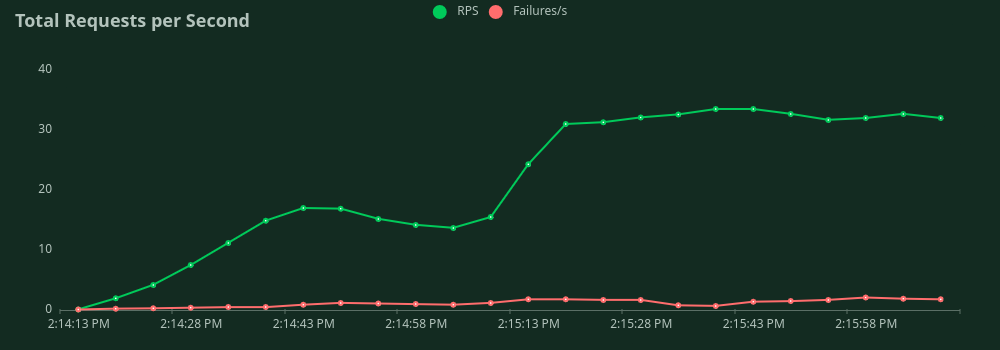
\includegraphics[width=0.9\textwidth]{requests-per-second.png}
				\end{subfigure}
				\vfill
				\begin{subfigure}[b]{\textwidth}
						\centering
						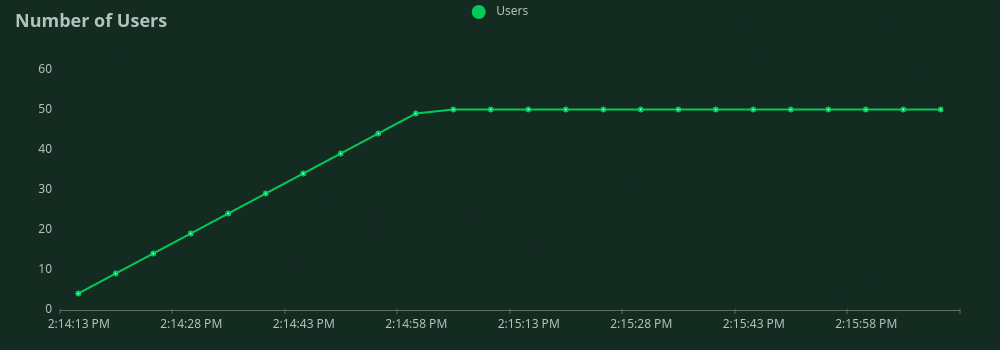
\includegraphics[width=0.9\textwidth]{number-of-users.png}
				\end{subfigure}
			\end{figure}
		}

		\only<3>{
			\vspace{-0.4cm}
			\hspace{-0.6cm} \cc{users: 50 | cpu: i7-8565U | ram: 8 GB DDR4}
			\begin{figure}[H]
				\centering
				\begin{subfigure}[b]{\textwidth}
						\centering
						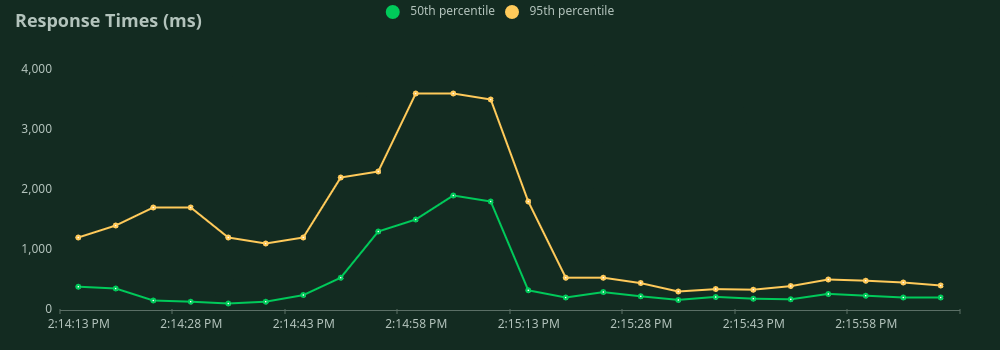
\includegraphics[width=0.9\textwidth]{response-times.png}
				\end{subfigure}
				\vfill
				\begin{subfigure}[b]{\textwidth}
						\centering
						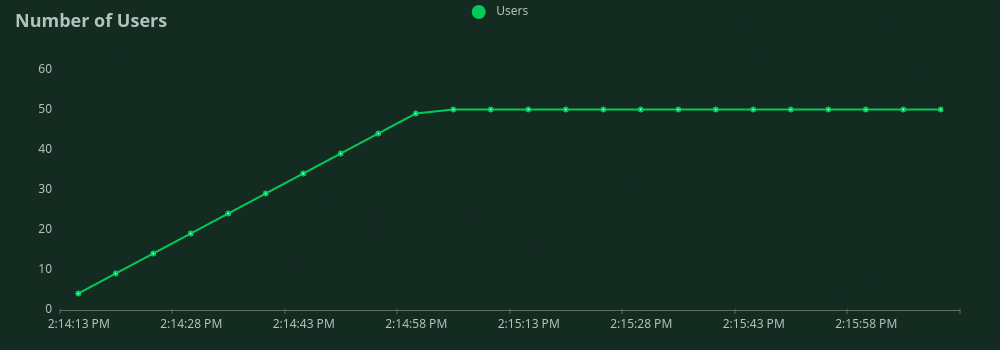
\includegraphics[width=0.9\textwidth]{number-of-users.png}
				\end{subfigure}
			\end{figure}
		}

\end{frame}
%-------------------------------------------------------------------------------
\subsection{Production Deployment}

\begin{frame}[t]
	\frametitle{Real-World Deployment}

	{
	\fontsize{8pt}{10pt}\selectfont
	\begin{table}[htb]
		\renewcommand{\arraystretch}{1.5} % Row height
		\centering
		\begin{tabular}{|c|c|c|c|c|}

			% Header (different color)
			\hline
			\rowcolor{boxcolor}
			\textbf{} &
			\textbf{On-premise} &
			\textbf{Iaas} &
			\textbf{Paas} &
			\textbf{Saas} \\ 

			% Rows
			\hline

		\end{tabular}
		\renewcommand{\arraystretch}{1} % Reset row height to default
	\end{table}
	}

\end{frame}

\begin{frame}[t]
	\frametitle{Real-World Deployment}

	{
	\fontsize{8pt}{10pt}\selectfont
	\begin{table}[htb]
		\renewcommand{\arraystretch}{1.5} % Row height
		\centering
		\begin{tabular}{|c|c|c|c|c|}

			% Header (different color)
			\hline
			\rowcolor{boxcolor}
			\textbf{} &
			\textbf{On-premise} &
			\textbf{Iaas} &
			\textbf{Paas} &
			\textbf{Saas} \\ 

			% Rows
			\hline
			\rowcolor{azure!30!white}
			\bft{Initial Investment} & High \faDollarSign\faDollarSign\faDollarSign & Medium \faDollarSign\faDollarSign & Low \faDollarSign & None \\
			\hline
			\rowcolor{azure!30!white}
			\bft{Set-Up Time} & Long \faClock\faClock\faClock & Medium \faClock\faClock & Short \faClock & None \\
			\hline

		\end{tabular}
		\renewcommand{\arraystretch}{1} % Reset row height to default
	\end{table}
	}

\end{frame}





\begin{frame}[t]
	\frametitle{Real-World Deployment}

	{
	\fontsize{8pt}{10pt}\selectfont
	\begin{table}[htb]
		\renewcommand{\arraystretch}{1.5} % Row height
		\centering
		\begin{tabular}{|c|c|c|c|c|}

			% Header (different color)
			\hline
			\rowcolor{boxcolor}
			\textbf{} &
			\textbf{On-premise} &
			\textbf{Iaas} &
			\textbf{Paas} &
			\textbf{Saas} \\ 

			% Rows
			\hline
			\rowcolor{azure!30!white}
			\bft{Initial Investment} & High \faDollarSign\faDollarSign\faDollarSign & Medium \faDollarSign\faDollarSign & Low \faDollarSign & None \\
			\hline
			\rowcolor{azure!30!white}
			\bft{Set-Up Time} & Long \faClock\faClock\faClock & Medium \faClock\faClock & Short \faClock & None \\
			\hline
			\rowcolor{green!30!white}
			\bft{Hardware Cost} & High \faDollarSign\faDollarSign\faDollarSign &
			None & None & None \\
			\hline
			\rowcolor{green!30!white}
			\bft{Maintenance Cost} & High \faDollarSign\faDollarSign\faDollarSign &
			Low \faDollarSign & None & None \\
			\hline
			\rowcolor{green!30!white}
			\bft{Fees Cost} & None & Low \faDollarSign & Medium
			\faDollarSign\faDollarSign & High \faDollarSign\faDollarSign\faDollarSign
			\\
			\hline

		\end{tabular}
		\renewcommand{\arraystretch}{1} % Reset row height to default
	\end{table}
	}

\end{frame}





\begin{frame}[t]
	\frametitle{Real-World Deployment}

	{
	\fontsize{8pt}{10pt}\selectfont
	\begin{table}[htb]
		\renewcommand{\arraystretch}{1.5} % Row height
		\centering
		\begin{tabular}{|c|c|c|c|c|}

			% Header (different color)
			\hline
			\rowcolor{boxcolor}
			\textbf{} &
			\textbf{On-premise} &
			\textbf{Iaas} &
			\textbf{Paas} &
			\textbf{Saas} \\ 

			% Rows
			\hline
			\rowcolor{azure!30!white}
			\bft{Initial Investment} & High \faDollarSign\faDollarSign\faDollarSign & Medium \faDollarSign\faDollarSign & Low \faDollarSign & None \\
			\hline
			\rowcolor{azure!30!white}
			\bft{Set-Up Time} & Long \faClock\faClock\faClock & Medium \faClock\faClock & Short \faClock & None \\
			\hline
			\rowcolor{green!30!white}
			\bft{Hardware Cost} & High \faDollarSign\faDollarSign\faDollarSign &
			None & None & None \\
			\hline
			\rowcolor{green!30!white}
			\bft{Maintenance Cost} & High \faDollarSign\faDollarSign\faDollarSign &
			Low \faDollarSign & None & None \\
			\hline
			\rowcolor{green!30!white}
			\bft{Fees Cost} & None & Low \faDollarSign & Medium
			\faDollarSign\faDollarSign & High \faDollarSign\faDollarSign\faDollarSign
			\\
			\hline
			\rowcolor{yellow!30!white}
			\bft{Scalability} & Limited \faRocket & High \faRocket\faRocket\faRocket &
			High \faRocket\faRocket\faRocket & High \faRocket\faRocket\faRocket \\
			\hline
			\rowcolor{yellow!30!white}
			\bft{Security} & Private & Shared & Your software & Vendor \\
			\hline
			\rowcolor{yellow!30!white}
			\bft{Control \& Privacy} & Full & Medium & Low & None \\
			\hline

		\end{tabular}
		\renewcommand{\arraystretch}{1} % Reset row height to default
	\end{table}
	}

\end{frame}
%-------------------------------------------------------------------------------
\section{Exercise 2}

\subsection{Assignment}

\begin{frame}
	
	\frametitle{Exercise 2 Assignment}

		\begin{itemize}

			\item The cluster must run \cc{k8s}
				\hspace{-0.4cm}
				\raisebox{-0.15cm}{
				
\includegraphics[width=0.8cm]{kubernetes-logo.png}}; one node is sufficient
			\item Pods must have probes to handle miss-behaviors \emoji{thermometer}
			\item Volumes must survive pod crash and accidental deletion
				\emoji{counterclockwise-arrows-button}
			\item Service must be accessible via IP or FQDN \emoji{globe-with-meridians}
			\item Databases or third-party services must run in their pod
				\emoji{card-file-box}

	\end{itemize}

\end{frame}
%-------------------------------------------------------------------------------
\subsection{Kubernetes Deployment}

\begin{frame}

	\frametitle{Kubernetes Deployment
	\hspace{-0.3cm}\raisebox{-0.2cm}{
\includegraphics[width=1cm]{kubernetes-logo.png}}}

	Deployment automated through \bft{provisioning scripts}:

	\begin{enumerate}
		\item \only<1->{Set-up a node using \cc{Vagrant} (\itt{alternative:
			\cc{Minikube}})}
		\item \only<2->{Install \cc{k8s} (and utilities) through provisioning
			script}
		\item \only<3->{Deploy \cc{MetalLB} through Helm chart}
		\item \only<4->{Deploy \cc{Ingress Nginx} controller through Helm chart}
		\item \only<5->{Apply \cc{PVs}, \cc{PVCs} and \cc{Secrets} for Nextcloud,
			PostgreSQL and Redis }
		\item \only<6->{Deploy \cc{Nextcloud} through Helm chart}
	\end{enumerate}

\end{frame}
\begin{frame}

	\frametitle{Kubernetes Deployment
	\hspace{-0.3cm}\raisebox{-0.2cm}{
\includegraphics[width=1cm]{kubernetes-logo.png}}}

	Simplified deployment scheme:
	\vspace{-0.5cm}
	
\begin{center}
\begin{adjustbox}{max width=\textwidth}
	\begin{tikzpicture}

		% Colors
		\definecolor{nextcloud}{HTML}{0082c9}
		\definecolor{postgres}{HTML}{0064a5}
		\definecolor{redis}{HTML}{a41e11}
		\definecolor{nginx}{HTML}{43a047}
		\definecolor{caddy}{HTML}{65d1ff}
		\definecolor{kubernetes}{HTML}{326ce5}

		% External User ---------------------------------------------------
		% \draw[-, line width=0.05cm, color=red] (-6, 0) -- (-4, 0);
		% \node (user) at (-6, 0) {
\includegraphics[width=1cm]{user-256.png}};
		% \node[anchor=south,
		% 			xshift=0cm,
		% 			yshift=-0.3cm,
		% 			color=kubernetes] 
		% 			at (user.south) {\fontsize{8pt}{10pt}\selectfont{Users}};

		% Node rectangle background ---------------------------------------
		\draw[fill=lightgray,
					opacity=0.5,
					line width=0.025cm,
					rounded corners=0.2cm
		] (-5, -3) rectangle (5, 3);
		\node at (-5, 3) {
\includegraphics[width=0.5cm]{master-256.png}};
		\node[color=kubernetes] at (-3.7, 3.2)
		{\fontsize{8pt}{10pt}\selectfont{Kubenetes Node}};

		% MetalLB Namespace (dotted rectangle) ----------------------------
		\draw[dotted,
					fill=darkblue,
					opacity=0.1,
					color=darkblue,
					line width=0.025cm,
					rounded corners=0.2cm
		] (-4.75, -2.75) rectangle (-3, 2.75);
		\draw[dotted,
					color=darkblue,
					line width=0.025cm,
					rounded corners=0.2cm
		] (-4.75, -2.75) rectangle (-3, 2.75);
		\node (mlb-ns) at (-4.5, 2.5) {
\includegraphics[width=0.4cm]{ns-256.png}};

		% External User ---------------------------------------------------
		\draw[-, line width=0.05cm, color=kubernetes] (-6, -0.15) -- (-4, -0.15);
		\node (user) at (-6, 0) {
\includegraphics[width=1cm]{user-256.png}};
		\node[anchor=south,
					xshift=0cm,
					yshift=-0.3cm,
					color=kubernetes] 
					at (user.south) {\fontsize{8pt}{10pt}\selectfont{Users}};

		\node[anchor=east,
					xshift=1.2cm,
					yshift=0cm,
					color=darkblue] 
					at (mlb-ns.east) {\fontsize{5pt}{10pt}\selectfont{metallb-system}};

		% Ingress Nginx Namespace (dotted rectangle) ----------------------
		\draw[dotted,
					fill=nginx,
					opacity=0.1,
					color=nginx,
					line width=0.025cm,
					rounded corners=0.2cm
		] (-2.75, -2.75) rectangle (-1, 2.75);
		\draw[dotted,
					color=nginx,
					line width=0.025cm,
					rounded corners=0.2cm
		] (-2.75, -2.75) rectangle (-1, 2.75);
		\draw[-, line width=0.05cm, color=kubernetes] (-4, -0.15) -- (-2, -0.15);
		\draw[-, line width=0.05cm, color=kubernetes] (-1.9, -0.15) -- (-1.9, 1.5);

		% MetalLb Speaker (ds)
		\node (speaker) at (-3.9, 0) {
\includegraphics[width=1cm]{ds-256.png}};
		\node[anchor=south,
					xshift=0cm,
					yshift=-0.3cm,
					color=kubernetes] 
					at (speaker.south) {\fontsize{6pt}{10pt}\selectfont{speaker}};


		\node (nginx-ns) at (-2.5, 2.5) {
\includegraphics[width=0.4cm]{ns-256.png}};
		\node[anchor=east,
					xshift=1.1cm,
					yshift=0cm,
					color=nginx] 
					at (nginx-ns.east) {\fontsize{5pt}{10pt}\selectfont{ingress-nginx}};

		% Ingress Nginx LoadBalancer (svc)
		\node (loadbalancer) at (-1.9, 0) {
\includegraphics[width=1cm]{svc-256.png}};
		\node[anchor=south,
					xshift=0cm,
					yshift=-0.3cm,
					color=kubernetes] 
					at (loadbalancer.south)
					{\fontsize{6pt}{10pt}\selectfont{nginx-ingress-svc}};
		\node[anchor=south,
					xshift=0cm,
					yshift=-0.5cm,
					color=kubernetes] 
					at (loadbalancer.south)
					{\fontsize{6pt}{10pt}\selectfont{\cc{LoadBalancer}}};

		% Ingress Controller (above)
		\draw[-, line width=0.05cm, color=kubernetes] (-1.9, 1.3) -- (0.8, 1.3);
		\node (controller) at (-1.9, 1.4) {
\includegraphics[width=1cm]{ing-256.png}};
		\node[anchor=north,
					xshift=0cm,
					yshift=+0.3cm,
					color=kubernetes] 
					at (controller.north)
					{\fontsize{6pt}{10pt}\selectfont{ingress-controller}};

		% Nextcloud Namespace (dotted rectangle) --------------------------
		\draw[dotted,
					fill=nextcloud,
					opacity=0.1,
					color=nextcloud,
					line width=0.025cm,
					rounded corners=0.2cm
		] (-0.75, -2.75) rectangle (4.75, 2.75);
		\draw[dotted,
					color=nextcloud,
					line width=0.025cm,
					rounded corners=0.2cm
		] (-0.75, -2.75) rectangle (4.75, 2.75);
		\node (nextcloud-ns) at (-0.5, 2.5) {
\includegraphics[width=0.4cm]{ns-256.png}};
		\node[anchor=east,
					xshift=0.85cm,
					yshift=0cm,
					color=nextcloud] 
					at (nextcloud-ns.east) {\fontsize{5pt}{10pt}\selectfont{nextcloud}};

		% Nextcloud Service (svc)
		\node (nextcloud-svc) at (0, 1.4) {
\includegraphics[width=1cm]{svc-256.png}};
		\node[anchor=south,
					xshift=0cm,
					yshift=-0.3cm,
					color=kubernetes] 
					at (nextcloud-svc.south)
					{\fontsize{6pt}{10pt}\selectfont{nextcloud-svc}};

		% Nextcloud Pod
		\draw[dotted,
					color=kubernetes,
					line width=0.025cm,
					rounded corners=0.2cm
		] (3, 2.2) rectangle (4.6, 0.5);
		\node at (4.5, 2.2) {
\includegraphics[width=0.4cm]{pvc-256.png}};
		\draw[draw=kubernetes,
					fill=kubernetes!30!white,
					line width=0.025cm,
					rounded corners=0.2cm
		] (0.8, 2.2) rectangle (3.3, -0.6);
		\node at (0.8, 2.2) {
\includegraphics[width=0.4cm]{pod-256.png}};

		\draw[draw=nginx,
					fill=nginx!30!white,
					line width=0.025cm,
					rounded corners=0.2cm
		] (0.9, 2.1) rectangle (3.2, 1.3);
		\node[color=black] at (1.5, 1.7) {\fontsize{6pt}{10pt}\selectfont{web
		server}};
		\node at (2.7, 1.7) {
\includegraphics[width=0.6cm]{Nginx_logo.png}};

		\draw[draw=nextcloud,
					fill=nextcloud!30!white,
					line width=0.025cm,
					rounded corners=0.2cm
		] (0.9, 1.2) rectangle (3.2, 0.4);
		\node[color=black] at (1.66, 0.8) {\fontsize{6pt}{10pt}\selectfont{nextcloud
		app}};
		\node at (2.7, 0.8) {
\includegraphics[width=0.6cm]{nextcloud-logo.png}};
		
		\draw[draw=nextcloud,
					fill=nextcloud!30!white,
					line width=0.025cm,
					rounded corners=0.2cm
		] (0.9, 0.3) rectangle (3.2, -0.5);
		\node[color=black] at (1.4, -0.1) {\fontsize{6pt}{10pt}\selectfont{cron
		jobs}};
		\node at (2.7, -0.1) {
\includegraphics[width=0.6cm]{nextcloud-logo.png}};

		% Redis Pod
		\draw[draw=kubernetes,
					fill=kubernetes!30!white,
					line width=0.025cm,
					rounded corners=0.2cm
		] (-0.3, -1.25) rectangle (2, -2.25);
		\node at (-0.3, -1.25) {
\includegraphics[width=0.4cm]{pod-256.png}};

		\draw[draw=redis,
					fill=redis!30!white,
					line width=0.025cm,
					rounded corners=0.2cm
		] (-0.2, -1.35) rectangle (1.9, -2.15);
		\node[color=black] at (0.5, -1.75) {\fontsize{6pt}{10pt}\selectfont{redis
		cache}};
		\node at (1.5, -1.75) {
\includegraphics[width=0.5cm]{redis-logo.png}};

		% Postgres Pod
		\draw[dotted,
					color=kubernetes,
					line width=0.025cm,
					rounded corners=0.2cm
		] (3.45, -1.5) rectangle (4.6, -0.3);
		\node at (4.5, -0.3) {
\includegraphics[width=0.4cm]{pvc-256.png}};
		\draw[draw=kubernetes,
					fill=kubernetes!30!white,
					line width=0.025cm,
					rounded corners=0.2cm
		] (2.3, -1.25) rectangle (4.6, -2.25);
		\node at (2.3, -1.25) {
\includegraphics[width=0.4cm]{pod-256.png}};

		\draw[draw=postgres,
					fill=postgres!30!white,
					line width=0.025cm,
					rounded corners=0.2cm
		] (2.4, -1.35) rectangle (4.5, -2.15);
		\node[color=black] at (3.1, -1.75)
		{\fontsize{6pt}{10pt}\selectfont{postgreSQL}};
		\node at (4.1, -1.75) {\includegraphics[width=0.5cm]{postgresql.png}};

		% PVs

		% nextcloud pv
		\node (nextcloud-pv) at (3.9, 1.5)
		{\includegraphics[width=0.8cm]{pv-256.png}};
		\node[anchor=south,
					xshift=0cm,
					yshift=-0.3cm,
					color=kubernetes] 
					at (nextcloud-pv.south)
					{\fontsize{6pt}{10pt}\selectfont{nextcloud-pv}};

		% postgresql pv
		\node (postgres-pv) at (4, -0.8)
		{\includegraphics[width=0.8cm]{pv-256.png}};

	\end{tikzpicture}
\end{adjustbox}
\end{center}


\end{frame}
%-------------------------------------------------------------------------------
\subsection{Kubernetes Deployment}
\begin{frame}
	\frametitle{Kubernetes Deployment Features and Advantages}

	Advantages:
	\begin{itemize}
		\checkeditem\ \bft{Scalability}: scale up or down pods or replicas
		\checkeditem\ \bft{Self-healing}: automatic pod restart in case of failure
		\checkeditem\ \bft{Resurces Management}: Horizontal Pod Autoscaler (HPA)
		\checkeditem\ \bft{Monitoring}: Startup, Readiness and Liveliness probes
		\checkeditem\ \bft{Rolling Updates}: zero update downtime	interruption
		\checkeditem\ \bft{Secrets Management}: for storing sensitive information
		\checkeditem\ \bft{Portability}: Kubernetes is cloud-agnostic
		\checkeditem\ \bft{Compatibility}: with many cloud providers
		\checkeditem\ \bft{Quick Deployment}: declarative \cc{yaml} files
	\end{itemize}

	Disadvantages:
	\begin{itemize}
		\negitem\ \bft{Complexity}: more complex than Docker
		\negitem\ \bft{Requirements}: $2$ GB RAM and $2$ CPUs
		\item[\empty]
	\end{itemize}

\end{frame}
%-------------------------------------------------------------------------------
\section{Exercise 3}

\subsection{Assignment}

\begin{frame}
	\frametitle{Exercise 3 Assignment}

% the cluster must run k8s; two nodes are necessary,
% the nodes must talk via either flannel or calico,
% the mpi operator must be installed,
% Create a container with the OSU benchmark on this page: https://mvapich.cse.ohio-state.edu/benchmarks/. More detailed instructions about compilation can be found here. This container must have a behavior as expected by the operator. Specialized containers must be created to compile and run the code. For example, follow the mpi-operator doc
% use the code to estimate the latency between the two nodes (by placing one worker per node) and at least one between collective operations. Compare these results with those when both pods are on the same node.

	\begin{itemize}

		\item The cluster must run \cc{k8s}
			\hspace{-0.4cm}
			\raisebox{-0.15cm}{
			\includegraphics[width=0.8cm]{kubernetes-logo.png}}; two node are
			necessary
		\item The nodes must talk via either \cc{flannel} or \cc{calico}
			\faNetworkWired
		\item The \cc{mpi-operator} must be installed 
		\item Create a container with the OSU benchmark	\emoji{chart-increasing}
		\item Estimate the latency between the two nodes \emoji{stopwatch}
	\end{itemize}

\end{frame}
%-------------------------------------------------------------------------------
\subsection{Double Node Structure}

\begin{frame}
	\frametitle{Exercise 3 Deployment and Benchmarks}

	Deployment steps:

	\begin{enumerate}
		\item \only<1->{Set-up $2$ nodes using \cc{Vagrant}}
		\item \only<2->{Install \cc{k8s}, copy \cc{admin.conf} file and add worker
			node with \cc{kubeadm join}}
		\item \only<3->{Install \cc{flannel} and set-up flannel network through
			Helm}
		\item \only<4->{Install \cc{mpi-operator} with specialized containers
			deployment and create a \cc{mpi-job} (\cc{yaml} file)}
	\end{enumerate}

	\only<5->{
		Conducted benchmarks:
		\begin{itemize}
			\item Point-to-point latency test
			\item Broadcast latency test
		\end{itemize}
	}

\end{frame}
%-------------------------------------------------------------------------------
\subsection{OSU Benchmark}

\begin{frame}
	\frametitle{OSU Benchmark: point-to-point latency test}
	\includegraphics[width=\textwidth]{p2p-one-node.pdf}
\end{frame}
\begin{frame}
	\frametitle{OSU Benchmark: point-to-point latency test}
	\includegraphics[width=\textwidth]{p2p-two-nodes.pdf}
\end{frame}
\begin{frame}
	\frametitle{OSU Benchmark: Broadcast latency test}
	\includegraphics[width=\textwidth]{broadcast-one-node.pdf}
\end{frame}
\begin{frame}
	\frametitle{OSU Benchmark: Broadcast latency test}
	\includegraphics[width=\textwidth]{broadcast-two-nodes.pdf}
\end{frame}
%-------------------------------------------------------------------------------
% \section{References}

% \nocite{*}

% \begin{frame}{References}
% \footnotesize % or \small or \tiny
% \bibliographystyle{plain}
% \bibliography{bibliography1}
% \end{frame}

\end{document}
